% -*- root: ../main.tex -*-
%!TEX root = ../main.tex
% this file is called up by main.tex
% content in this file will be fed into the main document
% vim:textwidth=80 fo=cqt

In   this    section,   the    quadratic   approximation   of    ionic   spatial
concentration,   that  underpins   the  electrolyte   model  in   many  improved
\gls{spm}  formulations  is  presented.  The  steps  involved  in  deriving  the
quadratic   approximation   is  detailed   in~\cref{subsec:quadraticmodelderiv}.
In~\cref{subsec:quadraticsimresultsanalysis},  an analysis  of  the weakness  of
this  model is  performed  based  on the  results  from  applying the  quadratic
approximation scheme. Mitigation of this critical drawback lead to this author's
decoupled  spatio-temporal electrolyte  concentration model  structure which  is
presented next in~\cref{sec:newelectrolytemodel}.

\subsection{Model derivation}\label{subsec:quadraticmodelderiv}

\begin{figure}[!htb]
    \captionsetup{singlelinecheck=off}
    \centering
    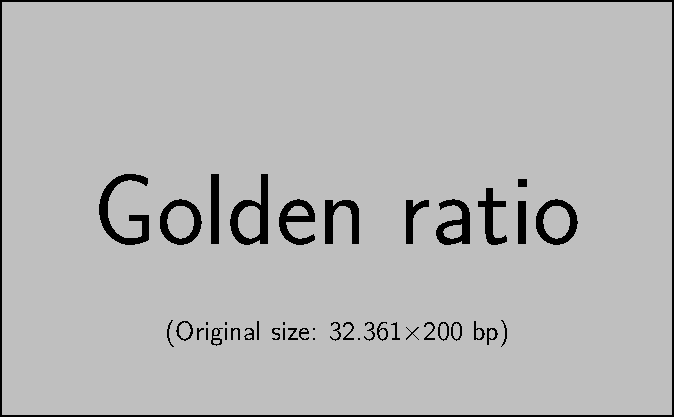
\includegraphics{placeholder_images/example-image-golden.pdf}
    \caption[Co-ordinate systems for quadratic approximation of
    electrolyte concentration]{Schematic diagram of the electrochemical sandwich
        consisting of
        \begin{enumerate*}[label=\itshape\alph*\upshape)]
            \item negative electrode,
            \item separator, and
            \item positive electrode
        \end{enumerate*} depicting the co-ordinate system used in deriving the
        quadratic approximation profile. The global spatial co-ordinate is $x
        \in \{0,l_\text{tot}\}$, where $l_\text{tot} = l_\text{neg} +
        l_\text{sep} + l_\text{pos}$. Local co-ordinate systems specific to each
        region are also defined. It should be noted that the positive
        electrode's local co-ordinate axis direction is reversed.}
    \label{fig:coordsquadapprox}
\end{figure}

The  schematic  in~\cref{fig:coordsquadapprox}  shows   the  definition  of  the
co-ordinate  systems  used  in  deriving the  polynomial  approximation  of  the
electrolyte concentration  profile. The globally defined  $x$ co-ordinate starts
at  the negative  current  collector  interface ($x=0$)  and  terminates at  the
positive  current  collector  interface  ($x =  l_\text{tot},\,  l_\text{tot}  =
l_\text{neg} +  l_\text{sep} +  l_\text{pos}$). Three local  co-ordinate systems
$z_\mu$  valid  only  within  their  respective regions  are  also  defined.  In
particular, it  must be  noted that  the direction  of the  local $z_\text{pos}$
co-ordinate axis is opposite to that of  the other two local co-ordinate axes as
well as the global co-ordinate axis. In subsequent usages, the suffix in $z_\mu$
is dropped and  the reader is advised  to infer the region of  validity from the
usage  context  which are  unambiguous  as  they  occur in  separate  equations.
Furthermore, the  notation of  the three regions  $\{\text{neg, sep,  pos}\}$ is
abbreviated  to $\{n,s,p\}$  respectively in  all mathematical  expressions. The
author  is convinced  that this  notation does  not detract  from following  the
derivations, but rather aids it by keeping the notations compact.

A  standard  quadratic expression  is  chosen  a  priori for  approximating  the
electrolyte concentration profile within each region.
\begin{alignat}{2}
    c_\ensub(z,t) & = a_2(t) z^2 + a_1(t) z + a_0(t) \qquad &  & 0 \le z \le l_\text{n}\label{eq:cenqquadstart}   \\
    c_\essub(z,t) & = a_5(t) z^2 + a_4(t) z + a_3(t) \qquad &  & 0 \le z \le l_\text{s}\label{eq:cesqquadstart}   \\
    c_\epsub(z,t) & = a_8(t) z^2 + a_7(t) z + a_6(t) \qquad &  & 0 \le z \le l_\text{p}\label{eq:cepqquadstart}
    \shortintertext{where     the    coefficient     vector    $\vec{a}(t)     =
    \vect{a_0(t),a_1(t),   \dots  ,a_8(t)}$   is  to   be  determined   at  each
    time-step\footnotemark.  Applying  boundary  conditions of  the  electrolyte
    diffusion equation from  the \gls{dfn} model~(refer~\cref{eq:dfnliquiddiff})
    to~\crefrange{eq:cenqquadstart}{eq:cepqquadstart},  it  is clear  that  $a_1
    =  0$ and  $a_7  = 0$.  Thus,~\crefrange{eq:cenqquadstart}{eq:cepqquadstart}
    become}
    c_\ensub      & = a_2 z^2 + a_0         \qquad          &  & 0 \le z \le l_\text{n}\label{eq:cenquadreduced} \\
    c_\essub      & = a_5 z^2 + a_4 z + a_3 \qquad          &  & 0 \le z \le l_\text{s}\label{eq:cesquadreduced} \\
    c_\epsub      & = a_8 z^2 + a_6         \qquad          &  & 0 \le z \le l_\text{p}\label{eq:cepquadreduced}
\end{alignat}
\footnotetext{In rest of  the equations, time-dependence of  the coefficients is
dropped from  the notation. It is  implicitly noted that they  are time-varying.
Similarly, spatio-temporal dependence of the electrolyte concentration functions
$c_\text{e,j}$ is omitted  in circumstances where such explicit  notation is not
crucial  for  understanding.} with  the  coefficient  vector being  modified  to
$\vec{a} = \vect{a_0,a_2, \dots ,a_6, a_8}$.

% -*- root: ../main.tex -*-
%!TEX root = ../main.tex
% this file is called up by main.tex
% content in this file will be fed into the main document
% vim:nospell textwidth=180 foldlevelstart=3 foldlevel=3 conceallevel=0

\begin{table}[!htb]
    \centering
    \caption[Electrolyte equations \& boundary conditions of \glsfmtshort{dfn} model in separator]{Electrolyte-specific governing equations and boundary conditions of the \glsfmtlong{dfn} model within the separator domain.}
    \label{tbl:dfnelectrolyteeqnsinsep}
    \begingroup
    \makeatletter\def\f@size{9.25}\check@mathfonts
    \addtolength{\jot}{0.875em}
    \begin{tabular*}{\textwidth}{@{} l c r l r @{}}
        \toprule
        \multicolumn{1}{c}{\small Region} & \small Governing equations & \multicolumn{2}{c}{\small Boundary conditions } & {} \\
        {} & {} & \multicolumn{2}{c}{\scriptsize $(l_\text{neg} \coloneqq l_\text{n},\, l_\text{sep} \coloneqq l_\text{s},\, l_\text{pos} \coloneq l_\text{p})$} \\
        \midrule
        \multicolumn{1}{l |}{{\rotatebox[origin=c]{90}{\makecell{\footnotesize Separator\\ \scriptsize $\delta \in \{\text{sep}\}$}}}} &
        $\begin{aligned}
            \vphantom{D_{\text{\tiny eff}_\text{n}}\!\! \! \!\, \diffp{c_\text{e}}{x}{\mathrlap{x = l^{-}_\text{n}}}} \varepsilon_\delta \diffp{c_\text{e}}{t} &=D_\effdelta  \diffp[2]{c_\text{e}}{x} \\[-0.75em]
            \vphantom{D_{\text{\tiny eff}_\text{s}}\!\! \! \!\, \diffp{c_\text{e}}{x}{\mathrlap{x=(l_{\text{n}} + l_\text{s})^{-}}}}\\[1.25em]
            \vphantom{\kappa_{\text{\tiny eff}_\text{n}}\!\! \! \!\, \diffp{c_\text{e}}{x}{\mathrlap{x = l^{-}_\text{n}}}\hspace{5mm} =\kappa_{\text{\tiny eff}_\text{s}}\!\!\!\!\,\diffp{c_\text{e}}{x}{\mathrlap{x = l^{+}_\text{n}}}} \frac{I}{A} &= \overline{\kappa}_\effdelta \left( \diffp[2]{\phi_\text{e}}{x} + \frac{2 R T}{F} (t^0_{+}-1)\diffp[2]{ \ln c_\text{e}}{x}\right) \\[-0.75em]
            \vphantom{\kappa_{\text{\tiny eff}_\text{s}}\!\! \! \!\, \diffp{c_\text{e}}{x}{\mathrlap{x=(l_{\text{n}} + l_\text{s})^{-}}}} \\
        \end{aligned}$ &
        $\begin{aligned}
    \vphantom{D_{\text{\tiny eff}_\text{n}}\!\! \! \!\, \diffp{c_\text{e}}{x}{\mathrlap{x = l^{-}_\text{n}}}} \qquad c_\text{e}\Bigr\rvert_{\mathrlap{x=l^{-}_\text{n}}}\hspace{5mm} &= c_\text{e}\Bigr\rvert_{\mathrlap{x=l^{+}_\text{n}}},\\[-0.75em]
     \vphantom{\kappa_{\text{\tiny eff}_\text{n}}\!\! \! \!\, \diffp{c_\text{e}}{x}{\mathrlap{x = l^{-}_\text{n}}}\hspace{5mm} =\kappa_{\text{\tiny eff}_\text{s}}\!\!\!\!\,\diffp{c_\text{e}}{x}{\mathrlap{x = l^{+}_\text{n}}}} c_\text{e}\Bigr\rvert_{\mathrlap{x=(l_{\text{n}} + l_\text{s})^{-}}}\hspace{5mm} &= c_\text{e}\Bigr\rvert_{\mathrlap{x=(l_{\text{n}} + l_\text{s})^{+}}},\\[1.25em]
 \vphantom{\kappa_{\text{\tiny eff}_\text{n}}\!\! \! \!\, \diffp{c_\text{e}}{x}{\mathrlap{x = l^{-}_\text{n}}}} \vphantom{\left( \diffp[2]{\phi_\text{e}}{x} + \frac{2 R T}{F} (t^0_{+}-1)\diffp[2]{ \ln c_\text{e}}{x}\right)} \phi_\text{e}\Bigr\rvert_{\mathrlap{x=l^{-}_\text{n}}}\hspace{5mm} &= \phi_\text{e}\Bigr\rvert_{\mathrlap{x=l^{+}_\text{n}}},\\[-0.75em]
 \vphantom{\kappa_{\text{\tiny eff}_\text{s}}\!\! \! \!\, \diffp{c_\text{e}}{x}{\mathrlap{x=(l_{\text{n}} + l_\text{s})^{-}}}} \phi_\text{e}\Bigr\rvert_{\mathrlap{x=(l_{\text{n}} + l_\text{s})^{-}}}\hspace{5mm} &= \phi_\text{e}\Bigr\rvert_{\mathrlap{x=(l_{\text{n}} + l_\text{s})^{-}}},\\
    \end{aligned}$ &
    $\begin{aligned}
        \quad D_{\text{\tiny eff}_\text{n}}\!\! \! \!\, \diffp{c_\text{e}}{x}{\mathrlap{x = l^{-}_\text{n}}}\hspace{5mm} &=D_{\text{\tiny eff}_\text{s}}\!\!\!\!\,\diffp{c_\text{e}}{x}{\mathrlap{x = l^{+}_\text{n}}}\\[-0.75em]
        D_{\text{\tiny eff}_\text{s}}\!\! \! \!\, \diffp{c_\text{e}}{x}{\mathrlap{x=(l_{\text{n}} + l_\text{s})^{-}}}\hspace{5mm} &=D_{\text{\tiny eff}_\text{p}}\!\!\!\!\,\diffp{c_\text{e}}{x}{\mathrlap{x=(l_{\text{n}} + l_\text{s})^{+}}}\\[1.25em]
        \vphantom{\left( \diffp[2]{\phi_\text{e}}{x} + \frac{2 R T}{F} (t^0_{+}-1)\diffp[2]{ \ln c_\text{e}}{x}\right)} \kappa_{\text{\tiny eff}_\text{n}}\!\! \! \!\, \diffp{c_\text{e}}{x}{\mathrlap{x = l^{-}_\text{n}}}\hspace{5mm} &=\kappa_{\text{\tiny eff}_\text{s}}\!\!\!\!\,\diffp{c_\text{e}}{x}{\mathrlap{x = l^{+}_\text{n}}}\\[-0.75em]
        \kappa_{\text{\tiny eff}_\text{s}}\!\! \! \!\, \diffp{c_\text{e}}{x}{\mathrlap{x=(l_{\text{n}} + l_\text{s})^{-}}}\hspace{5mm} &=\kappa_{\text{\tiny eff}_\text{p}}\!\!\!\!\,\diffp{c_\text{e}}{x}{\mathrlap{x=(l_{\text{n}} + l_\text{s})^{+}}}\\
    \end{aligned}$ &
    $\begin{aligned}
        \vphantom{D_{\text{\tiny eff}_\text{n}}\!\! \! \!\, \diffp{c_\text{e}}{x}{\mathrlap{x = l^{-}_\text{n}}}} \quad \refstepcounter{equation}(\theequation)\label{eq:liquiddiffnsep} \\[-0.75em]
        \vphantom{D_{\text{\tiny eff}_\text{s}}\!\! \! \!\, \diffp{c_\text{e}}{x}{\mathrlap{x=(l_{\text{n}} + l_\text{s})^{-}}}}\\[1.25em]
        \vphantom{\kappa_{\text{\tiny eff}_\text{n}}\!\! \! \!\, \diffp{c_\text{e}}{x}{\mathrlap{x = l^{-}_\text{n}}}} \vphantom{\left( \diffp[2]{\phi_\text{e}}{x} + \frac{2 R T}{F} (t^0_{+}-1)\diffp[2]{ \ln c_\text{e}}{x}\right)} \refstepcounter{equation}(\theequation) \label{eq:liquidpotentialsep}\\[-0.75em]
        \vphantom{\kappa_{\text{\tiny eff}_\text{s}}\!\! \! \!\, \diffp{c_\text{e}}{x}{\mathrlap{x=(l_{\text{n}} + l_\text{s})^{-}}}}
    \end{aligned}$
    \\
    \bottomrule
\end{tabular*}
\endgroup
\end{table}



\Cref{tbl:dfnelectrolyteeqnsinsep} lists  the equations and  boundary conditions
for  phenomena  describing  electrolyte  diffusion  and  charge  balance  within
the separator  domain. \Cref{eq:liquiddiffnsep} and~\cref{eq:liquidpotentialsep}
are  obtained  by  applying  the  corresponding  electrolyte  equations  of  the
\gls{dfn}  model  (see~\cref{eq:dfnliquiddiff}  and~\cref{eq:dfnliquidpotential}
respectively) to the separator region.

Applying  the  continuity  and  flux  boundary  conditions  of  the  electrolyte
diffusion  equation from~\cref{eq:liquiddiffnsep}  at both  separator
interfaces
\begin{alignat}{2}
    a_2 l^2_\text{n} + a_0                      & = \hphantom{-}a_3 \qquad                    &  & \text{\footnotesize (continuity at neg/sep interface)} \label{eq:cecontinuitynegsep} \\
    a_5 l^2_\text{s} + a_4 l_\text{s} + a_3     & = \hphantom{-}a_8 l^2_\text{p} + a_6 \qquad &  & \text{\footnotesize (continuity at sep/pos interface)}                               \\
    2 a_2 l_\text{n} D_\effn                    & = \hphantom{-}a_4 D_\effs \qquad            &  & \text{\footnotesize (flux b.c.\ at neg/sep interface)}                               \\
    \left(2 a_5 l_\text{s} + a_4\right) D_\effs & = -2 a_8 l_\text{p} D_\effp \qquad          &  & \text{\footnotesize (flux b.c.\ at sep/pos interface)}\label{eq:quadcefluxseppos}
\end{alignat}
Note that the negative sign in~\cref{eq:quadcefluxseppos} is due to the specific
choice of the co-ordinate system used  for the positive electrode region. Due to
this,  fluxes  at  the  separator/positive  electrode  interface  have  opposing
directions.

Let  $Q_\text{e,j}$  denote  the  number  of moles  of  \ch{Li^+}  ions  in  the
electrolyte per  unit cross-sectional  area within each  region $\jinnegseppos$.
This is  computed as  the product  of
\begin{enumerate*}[label=\emph{\alph*})]
    \item the porosity and
    \item spatial integral of the concentration function
\end{enumerate*}
\ie{}  $ Q_\text{e,j}  =  \varepsilon_j \int_0^{l_j}  c_{\text{e},j}(z) \,dz  $.
Applying this to \crefrange{eq:cenquadreduced}{eq:cepquadreduced}
\begin{align}
    Q_\text{e,n} &= \varepsilon_\text{n} \left( \frac{1}{3} a_2 l^3_\text{n} + a_0 l_\text{n}\right)\\
    Q_\text{e,s} &= \varepsilon_\text{s} \left( \frac{1}{3} a_5 l^3_\text{s} + \frac{1}{2} a_4 l^2_\text{s} + a_3 l_\text{s}\right)\\
    Q_\text{e,p} &= \varepsilon_\text{p} \left( \frac{1}{3} a_8 l^3_\text{p} + a_6 l_\text{p}\right) \label{eq:Qepbyintegration}
\end{align}

At this stage,  $Q_{\text{e},j}(t)$ are unknown. Since  these are time-dependent
functions,  the  derivation  naturally  progresses  towards  seeking  a  set  of
\glspl{ode} that describe a relationship  for their time evolution. We transform
the  second   order  \glspl{ode}  of~\cref{eq:dfnliquiddiff}   (for  electrodes)
and~\cref{eq:liquiddiffnsep}   (for  separator)   to   their  respective   local
co-ordinates and integrate  once along the thickness of  each region. Performing
this sequence of steps for the negative electrode region
\mathleft
\begin{equation}
\begin{WithArrows}[b]
    \varepsilon_\text{n} \int_0^{l_\text{n}} \left(\diffp*{c_\ensub(z,t)}{t}\right)\, dz &= \int_0^{l_\text{n}} \left(\diffp{}{z}\left(D_\effn \diffp{c_\ensub}{z} \right) + (1 - t^0_\text{+}) a_\snsub j_\text{n}\right)\, dz \Arrow[tikz={text width=3.4cm}]{transposing integration \& differentiation operations in the \glsfmtshort{lhs}} \\
    \varepsilon_\text{n} \diffp*{\int_0^{l_\text{n}} c_\ensub(z,t)}{t}\, dz &=
    \int_0^{l_\text{n}} \left(\diffp{}{z}\left(D_\effn \diffp{c_\ensub}{z}
    \right) + (1 - t^0_\text{+}) a_\snsub j_\text{n}\right)\, dz
    \Arrow[tikz={text width=3.4cm}]{apply time-derivative operator to the whole \glsfmtshort{lhs}}\\
    \diffp*{\left(\tikzmark{StartBraceA}\varepsilon_\text{n} \int_0^{l_\text{n}}
    c_\ensub(z,t)\, dz\tikzmark{EndBraceA}\right)}{t} &=  \int_0^{l_\text{n}}
    \left(\diffp{}{z}\left(D_\effn \diffp{c_\ensub}{z} \right) + (1 -
    t^0_\text{+}) a_\snsub j_\text{n}\right)\, dz \Arrow[tikz={text
width=3.4cm}]{apply integral to the \glsfmtshort{rhs}}\\
    \diff*{Q_\text{e,n}(t)}{t} &= D_\effn \diffp{c_\ensub}{z}{\mathrlap{z=l_\text{n}}} + (1 - t^0_\text{+}) a_\snsub \int_0^{l_\text{n}} j_\text{n}\, dz
\end{WithArrows}
\label{eq:negliionmolestoreduce}
\end{equation}
\mathcenter
\InsertUnderBrace[draw=black][aspect=0.26]{StartBraceA}{EndBraceA}{} % https://tex.stackexchange.com/questions/68526/asymmetric-overbrace

% \blindtext
% \AddToShipoutPicture*{\ShowFramePicture}

Performing     the     identical     sequence     of     operations     starting
from~(\cref{eq:liquiddiffnsep}) for  the separator and~(\cref{eq:dfnliquiddiff})
for the positive electrode yields
\begin{align}
    \diff*{Q_\text{e,s}(t)}{t} &= D_\effs \diffp{c_\essub}{z}{\mathrlap{z=l_\text{s}}} \label{eq:sepliionmolestoreduce}\\
    \diff*{Q_\text{e,p}(t)}{t} &= D_\effp \diffp{c_\epsub}{z}{\mathrlap{z=l_\text{p}}} + (1 - t^0_\text{+}) a_\spsub \int_0^{l_\text{p}} j_\text{p}\, dz\label{eq:posliionmolestoreduce}
\end{align}

In    order    to   evaluate    the    integral    term   in    the    \gls{rhs}
of~\cref{eq:negliionmolestoreduce}    and~\cref{eq:posliionmolestoreduce},   the
solid  phase  charge  conservation  equation~(\cref{eq:solidchargeconserve})  is
integrated  along the  local  co-ordinate  axis of  the  negative electrode  and
positive electrode respectively
\begin{align}
    \int_0^{l_\text{n}} j_\text{n}\, dz & =  \frac{I}{a_\snsub A F} \label{eq:negfluxintegral}\\
    \int_0^{l_\text{p}} j_\text{p}\, dz & =  \frac{-I}{a_\spsub A F}\label{eq:posfluxintegral}
\end{align}

Substituting~\crefrange{eq:negfluxintegral}{eq:posfluxintegral}
into~\crefrange{eq:negliionmolestoreduce}{eq:posliionmolestoreduce}
respectively
\begin{align}
    \diff*{Q_\text{e,s}}{t} &= D_\effn \diffp{c_\ensub}{z}{\mathrlap{z=l_\text{n}}} - (1 - t^0_\text{+}) \cancel{a_\snsub} \frac{I}{\cancel{a_\snsub} A F} \\
    \diff*{Q_\text{e,p}}{t} &= D_\effp \diffp{c_\epsub}{z}{\mathrlap{z=l_\text{p}}} - (1 - t^0_\text{+}) \cancel{a_\spsub} \frac{-I}{\cancel{a_\snsub} A F}
\end{align}

which leads to the general expressions  for the cross-sectional molar density of
\ch{Li^+} ions in each of the three regions as
\begin{align}
    \diff*{Q_\text{e,n}}{t} & = D_\effn \diffp{c_\ensub}{z}{\mathrlap{z=l_\text{n}}} + (1 - t^0_\text{+}) \frac{I}{A F} \label{eq:negliionmolesgen} \\
    \diff*{Q_\text{e,s}}{t} & = D_\effs \diffp{c_\essub}{z}{\mathrlap{z=l_\text{s}}} \label{eq:sepliionmolesgen}                                             \\
    \diff*{Q_\text{e,p}}{t} & = D_\effp \diffp{c_\epsub}{z}{\mathrlap{z=l_\text{p}}} - (1 - t^0_\text{+}) \frac{I}{A F}\label{eq:posliionmolesgen}
    \intertext{Substituting the assumed quadratic expressions for electrolyte concentrations in
        each of the three region, \ie{}~\crefrange{eq:cenquadreduced}{eq:cepquadreduced}
    in the above system,\ie{}~\crefrange{eq:negliionmolesgen}{eq:posliionmolesgen}}
    \diff*{Q_\text{e,n}}{t} & = 2 a_2 l_\text{n} D_\effn + (1 - t^0_\text{+}) \frac{I}{A F} \label{eq:negliionmolesquadratic}                                \\
    \diff*{Q_\text{e,s}}{t} & = 2 a_5 l_\text{s} D_\effs                                                                                                     \\
    \diff*{Q_\text{e,p}}{t} & = 2 a_8 l_\text{p} D_\effp - (1 - t^0_\text{+}) \frac{I}{A F} \label{eq:posliionmolesquadratic}
\end{align}
The  initial  ionic  concentration  in  the electrolyte  are  identical  in  all
three  regions  of  the  cell, assuming  equilibrium  starting  conditions~\ie{}
$c_{\text{e,0}_j} = c_\text{e,0}, \jinnsp$. Hence the initial number of moles of
\ch{Li^+} per unit area in each of the three regions is given by
\begin{align}
    Q_\text{e,n}(0) & = \varepsilon_\text{n} c_\text{e,0} l_\text{n} \label{eq:Qeninit}\\
    Q_\text{e,s}(0) & = \varepsilon_\text{s} c_\text{e,0} l_\text{s}\\
    Q_\text{e,p}(0) & = \varepsilon_\text{p} c_\text{e,0} l_\text{p} \label{eq:Qepinit}\\
    \shortintertext{and the initial coefficient vector which satisfies the system
    equations is obtained as}
    \begin{bmatrix}
        a_0 \\
        a_2 \\
        a_3 \\
        a_4 \\
        a_5 \\
        a_6 \\
        a_8
    \end{bmatrix} & = \begin{bmatrix}
        c_\text{e,0} \\
        0 \\
        c_\text{e,0} \\
        0 \\
        0 \\
        c_\text{e,0} \\
        0
    \end{bmatrix} \label{eq:coeffinit}
\end{align}

The             system             of             three             \glspl{ode},
\eqref{eq:negliionmolesquadratic}--\eqref{eq:posliionmolesquadratic}    together
with  \crefrange{eq:Qeninit}{eq:Qepinit}  representing the  initial  conditions,
form   an    \gls{ivp}.   \Crefrange{eq:cecontinuitynegsep}{eq:Qepbyintegration}
represent a square system of seven linear algebraic equations with seven unknown
coefficients  which  needs to  be  solved  at  each time-step.  These  algebraic
constraints coupled with the aforementioned \gls{ivp} form a \gls{dae} system.

There are now two choices for proceeding  with solution of the system. The naive
approach  would be  to  solve  the \gls{dae}  using  advanced \gls{dae}  solvers
specially  designed  to  handle  index-1 semi-explicit  systems  such  as  DASSL
or  DASPK. For  start-stop  type  of input  currents  with discontinuities,  the
consistent initialisation of algebraic conditions and derivatives is numerically
challenging.  All   \gls{dae}  solvers  typically  use   adaptive  time-stepping
algorithms.  The  feasibility of  using  such  a  complex scheme  for  real-time
computation is questionable. On the other hand, the overall system can be viewed
as composed of two numerical subsystems ---
\begin{enumerate*}[label=\emph{\alph*})]
    \item an independent \gls{ode} system, and
    \item an independent algebraic system
\end{enumerate*}
with both these  systems running back to back in  succession using solution from
the previous time-step.

To clarify the  sequence of operations, in  order to bootstrap the  model, it is
required  to compute  $Q_{\text{e},j}(t)$ in  all three  regions. The  \gls{ode}
system is  integrated for one time-step  by retaining the coefficients  at their
initial  value. The  $Q_{\text{e},j}(t)$  thus solved  is  substituted into  the
algebraic system to yield the updated value of the coefficient vector $\vec{a}(t
= t_k)$. This new  value of the coefficient vector is  substituted back into the
\gls{ode} system and  the process continues. Although  the continuous simulation
of  the overall  \gls{dae} is  not possible,  this scheme  is pragmatic  from an
engineering viewpoint  as the periodic  pauses needed to update  the intertwined
sub-systems translate naturally  into fixed time-steps and is  well-suited for a
\gls{bms} controller operating at a fixed sample rate. This is also an effective
workaround  to  mitigate the  complexities  of  having  to implement  and  solve
\glspl{dae} in real time.

% need to write algorithm
The   simulation   results   of   the   quadratic   approximation   scheme   and
the   analysis   of   its   strengths   and   weaknesses   is   presented   next
in~\cref{subsec:quadraticsimresultsanalysis}.

\subsection{Numerical implementation, simulation results and analysis}\label{subsec:quadraticsimresultsanalysis}

From an analysis point of view,  the quadratic approximation model for computing
the spatio-temporal evolution of electrolyte concentration can be simulated as a
standalone subsystem, and  hence can be implemented numerically  as a standalone
module  as  shown  in~\cref{alg:quadraticce}.  In practice,  this  modular  code
is  embedded  as  a  subroutine  within  the  main  \gls{spm}  algorithm  listed
in~\cref{alg:disctimespm}.

% -*- root: ../main.tex -*-
%!TEX root = ../main.tex
% this file is called up by main.tex
% content in this file will be fed into the main document
% vim:nospell

\begin{algorithm}[!htbp]
    \caption{Quadratic approximation model for spatio-temporal electrolyte concentration}\label{alg:quadraticce}
    \begin{algorithmic}[1]
        \Require Load profile \Comment{\eg{} a \texttt{csv} file of $t$ vs. C-rate}
        \Require Electrolyte model parameter set  \Comment{\eg{} stored in a struct \texttt{ceparams}}
        \Userdata $ t_\text{f}$,  sample rate $T_s, c_\text{e,init}$
        \Function{QuadraticElectrolyteModel}{}
            \State $Q_\text{e,init}$
            \State \vdots
            \State
            \State
            \State
            \State $V_\text{cell}[1] \gets \textsc{ComputeCellVoltage}(\textbf{x}[1],I[1],\texttt{params})$ \Comment{from direct feedthrough}
            \For{$k \gets 2 : N_\text{max}$}
                \State $I[k] \gets $ interpolate from profile using \gls{zoh}
                \State Solve continuous-time equation~\cref{eq:threestatesmatrixvec} \Comment{solver IC set to $x[k-1]$}
                \State $\mathbf{x}[k] \gets $ last time-entry  vector of soln.\  matrix \Comment{from an adaptive solver \eg{} MATLAB's \texttt{ode45}}
                \State Compute $z[k]$ as per~\cref{eq:soccomputation}
                \State $V_\text{cell} \gets \textsc{ComputeCellVoltage}(\textbf{x}[k],I[k],\texttt{param}) $
                \If {$z[k] \text{ or } V_\text{cell}[k]$ exceeded cut-off limits}
                    \State $k \gets k - 1$ \Comment{data from last  step is invalid}
                    \State \textit{break};
                \EndIf
            \EndFor
        \EndFunction

        \OutputEqn{\textbf{x}, I, \texttt{params}}
            \State Compute $c_\snegsurf$ as per~\cref{eq:csurfnegfromcavgneg}
            \Comment{consider saturating \ie{} $c_\snegmin \le c_\snegsurf \le
            c_\snegmax$}
            \State Compute $\mean{c}_\spos$ as per~\cref{eq:csposbulkfromcsnegbulk}
            \State Compute $c_\spossurf$ as per~\cref{eq:csurfposfromcavgpos}
            \State Compute $V_\text{cell}$ as per~\cref{eq:spmbasicoutputvoltagefinal}
        \EndOutputEqn%
    \end{algorithmic}
\end{algorithm}


\begin{figure}[!htb]
    \centering
    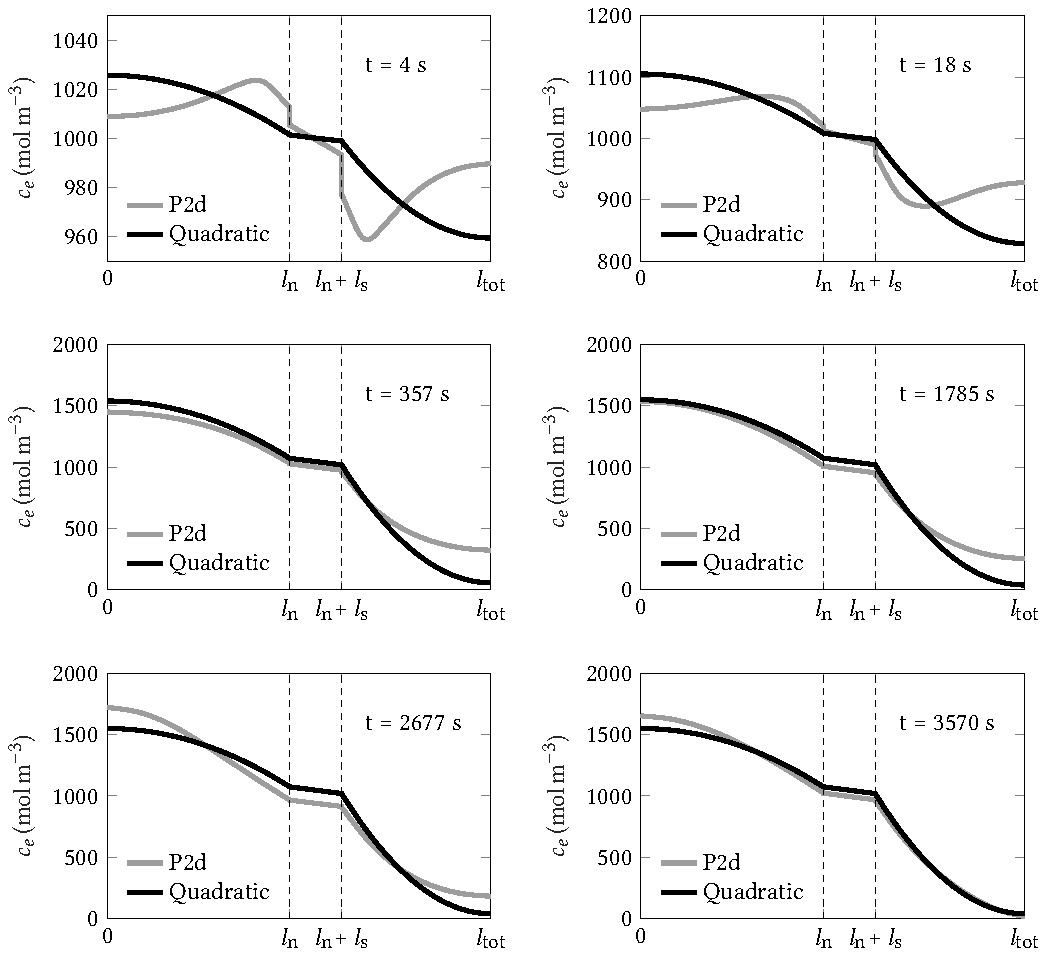
\includegraphics[width=\textwidth]{4/figures/quadratic_ce_approx_spatial_1C.pdf}
    \caption[Spatial distribution of electrolyte concentration for 1C
    discharge]{Spatial distribution of ionic concentration in electrolyte along
        cell thickness at various snapshots of time for a 1C discharge. The
        concentration profile obtained from simulating the \glsfmtshort{p2d}
        model is used as the reference. The performance of the quadratic model
        is quite poor during the initial transient duration, but improves over
    time as a quasi-steady state is reached.}
        \label{fig:spatialionicconc1C}
\end{figure}

\Cref{fig:spatialionicconc1C} shows  the spatial distribution of  \ch{Li^+} ions
in electrolyte  along the  thickness of  the cell at  various snapshots  of time
obtained by simulation  of the \gls{p2d} and the  quadratic approximation models
using a  1C discharge current. The  \gls{p2d} model's response is  considered as
the reference benchmark.  During the initial transient  phase, the concentration
profile within each electrode region exhibits a characteristic inflection point.
During this phase,  the concentration profile computed by  the parabolic profile
exhibits  a  large deviation  in  terms  of  percentage  error at  each  spatial
location. However, with the passage of time, as a \gls{qss} is established, this
inflection point flattens out, and the quadratic approximation becomes closer to
the  true  concentration value  at  each  spatial  location. Similar  trends  in
behaviour is  exhibited for discharge and  charging at higher C-rates  and these
results are  therefore omitted here  in the  interest of keeping  the discussion
succinct.

It  is important  to  note that  while having  a  spatial concentration  profile
is  useful,  as  seen  in~\cref{eq:electrolytepdwithce}, it  is  the  values  of
concentration  at   the  \emph{current  collector  interfaces}   that  are  most
influential in  computation of the  electrolyte overpotential and hence,  in the
voltage accuracy of the enhanced \gls{spm}. Thus, it is important to obtain this
alternative  perspective  of time-evolution  of  the  concentration at  the  two
current collectors.

% % This file was created by matlab2tikz.
%
\definecolor{mycolor1}{rgb}{0.61569,0.61569,0.61569}%
\definecolor{mycolor2}{rgb}{0.38824,0.38824,0.38824}%
%
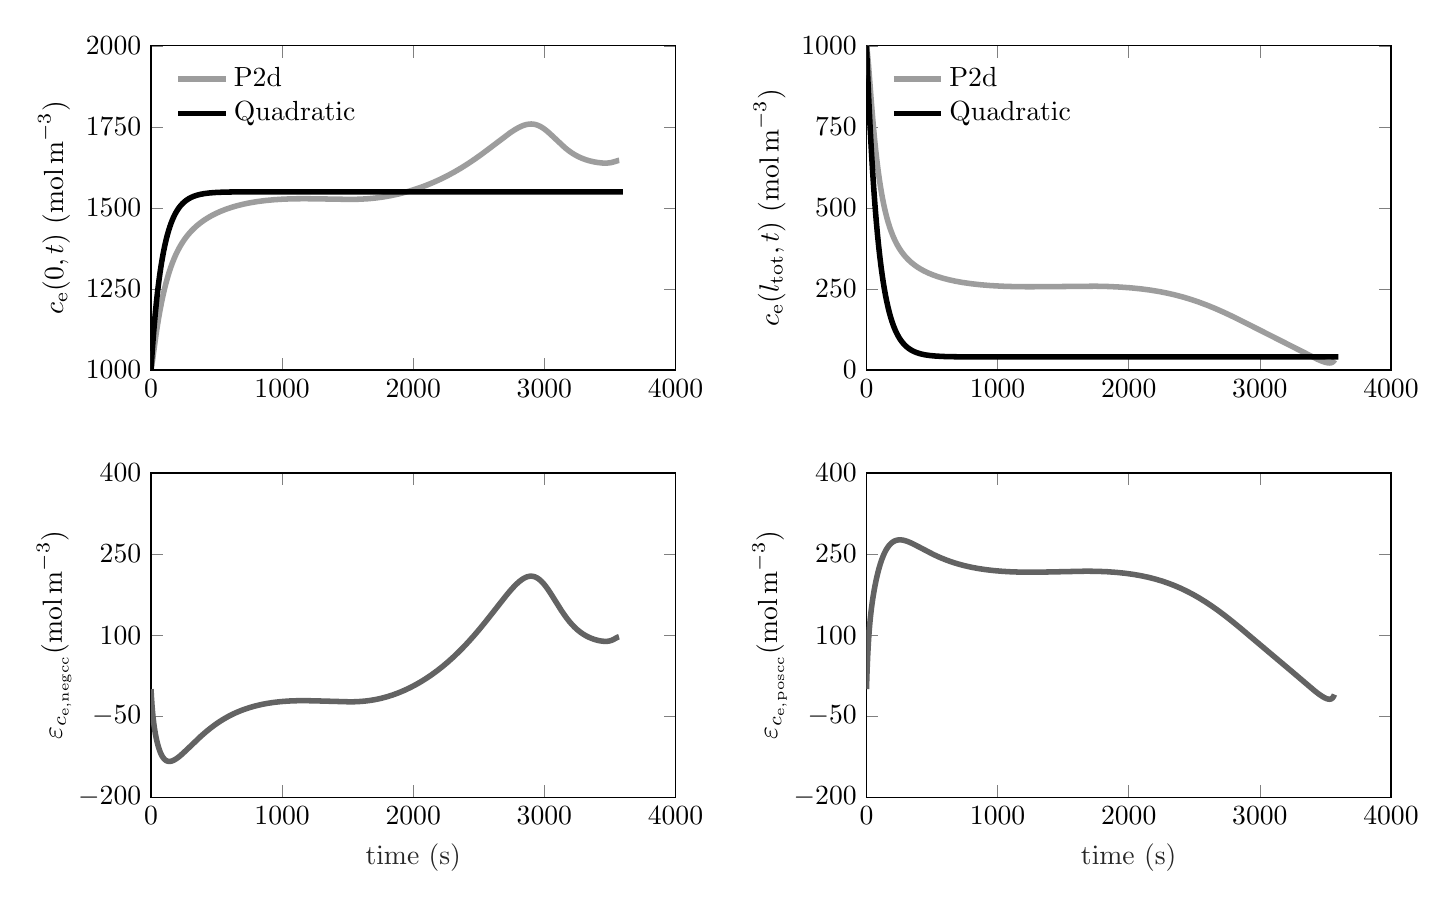
\begin{tikzpicture}

\begin{axis}[%
width=66.611mm,
height=41.169mm,
at={(0mm,54.255mm)},
scale only axis,
xmin=0,
xmax=4000,
xtick={0,1000,2000,3000,4000},
ymin=1000,
ymax=2000,
ytick={1000, 1250, 1500, 1750, 2000},
ylabel style={font=\color{white!15!black}},
ylabel={$c_{\mathrm{e}}(0,t)\  (\mathrm{mol\, m}^{-3})$},
axis background/.style={fill=white},
legend style={at={(0.03,0.97)}, anchor=north west, legend cell align=left, align=left, fill=none, draw=none},
scaled ticks=false,,
xticklabel style={/pgf/number format/1000 sep=, /pgf/number format/precision=0,/pgf/number format/fixed,/pgf/number format/fixed zerofill,},yticklabel style={/pgf/number format/1000 sep=, /pgf/number format/precision=2, /pgf/number format/fixed, }, ylabel absolute,
]
\addplot [color=mycolor1, line width=2.0pt]
  table[row sep=crcr]{%
0	1000\\
5	1011.48\\
11	1027.59\\
21	1057.49\\
37	1104.91\\
48	1134.7\\
59	1161.96\\
70	1186.88\\
81	1209.68\\
92	1230.58\\
103	1249.75\\
115	1268.89\\
127	1286.35\\
139	1302.29\\
151	1316.85\\
164	1331.24\\
177	1344.33\\
191	1357.13\\
205	1368.74\\
220	1380.03\\
235	1390.26\\
251	1400.15\\
268	1409.67\\
286	1418.78\\
306	1427.9\\
327	1436.51\\
350	1444.98\\
375	1453.22\\
402	1461.17\\
431	1468.78\\
462	1476.02\\
496	1483.04\\
532	1489.59\\
571	1495.79\\
613	1501.57\\
658	1506.88\\
706	1511.66\\
758	1515.95\\
814	1519.67\\
874	1522.77\\
939	1525.24\\
1009	1527.01\\
1086	1528.08\\
1173	1528.39\\
1278	1527.85\\
1528	1526.17\\
1597	1526.87\\
1658	1528.35\\
1715	1530.6\\
1771	1533.68\\
1827	1537.64\\
1883	1542.48\\
1939	1548.2\\
1994	1554.7\\
2049	1562.08\\
2103	1570.21\\
2156	1579.06\\
2208	1588.63\\
2260	1599.08\\
2311	1610.22\\
2362	1622.26\\
2413	1635.18\\
2465	1649.26\\
2520	1665.05\\
2583	1684.08\\
2737	1731.1\\
2771	1740.21\\
2799	1746.81\\
2823	1751.59\\
2844	1754.92\\
2864	1757.23\\
2883	1758.51\\
2901	1758.83\\
2918	1758.25\\
2935	1756.8\\
2952	1754.45\\
2969	1751.22\\
2987	1746.9\\
3006	1741.44\\
3028	1734.15\\
3055	1724.21\\
3157	1685.62\\
3184	1676.93\\
3209	1669.78\\
3234	1663.51\\
3260	1657.9\\
3287	1652.99\\
3315	1648.78\\
3345	1645.13\\
3377	1642.1\\
3411	1639.77\\
3443	1638.44\\
3470	1638.13\\
3493	1638.72\\
3513	1640.11\\
3533	1642.39\\
3567	1646.55\\
3570.66	1646.75\\
};
\addlegendentry{P2d}

\addplot [color=black, line width=2.0pt]
  table[row sep=crcr]{%
0	1000\\
8	1050.12\\
16	1094.78\\
24	1134.89\\
33	1175.42\\
42	1211.76\\
51	1244.43\\
60	1273.87\\
69	1300.43\\
78	1324.41\\
87	1346.06\\
96	1365.63\\
105	1383.31\\
115	1400.97\\
125	1416.76\\
135	1430.87\\
145	1443.48\\
155	1454.75\\
166	1465.77\\
177	1475.52\\
188	1484.13\\
200	1492.39\\
212	1499.61\\
225	1506.41\\
239	1512.7\\
254	1518.44\\
270	1523.58\\
287	1528.12\\
306	1532.26\\
327	1535.93\\
351	1539.19\\
378	1541.94\\
410	1544.29\\
448	1546.18\\
496	1547.65\\
561	1548.73\\
660	1549.4\\
858	1549.69\\
2037	1549.73\\
3599	1549.73\\
};
\addlegendentry{Quadratic}

\end{axis}

\begin{axis}[%
width=66.611mm,
height=41.169mm,
at={(90.867mm,54.255mm)},
scale only axis,
xmin=0,
xmax=4000,
xtick={0,1000,2000,3000,4000},
ymin=0,
ymax=1000,
ytick={   0,  250,  500,  750, 1000},
ylabel style={font=\color{white!15!black}},
ylabel={$c_\mathrm{e}(l_\mathrm{tot},t)\ (\mathrm{mol\, m}^{-3})$},
axis background/.style={fill=white},
legend style={at={(0.03,0.97)}, anchor=north west, legend cell align=left, align=left, fill=none, draw=none},
scaled ticks=false,,
xticklabel style={/pgf/number format/1000 sep=, /pgf/number format/precision=0,/pgf/number format/fixed,/pgf/number format/fixed zerofill,},yticklabel style={/pgf/number format/1000 sep=, /pgf/number format/precision=2, /pgf/number format/fixed, }, ylabel absolute,
]
\addplot [color=mycolor1, line width=2.0pt]
  table[row sep=crcr]{%
0	1000\\
2	995.472\\
5	986.098\\
9	970.517\\
15	942.691\\
24	895.759\\
42	801.533\\
52	754.003\\
62	710.838\\
71	675.655\\
80	643.719\\
89	614.777\\
98	588.56\\
107	564.806\\
116	543.269\\
126	521.666\\
136	502.245\\
146	484.76\\
156	468.98\\
166	454.708\\
177	440.546\\
188	427.799\\
200	415.302\\
212	404.087\\
225	393.188\\
238	383.416\\
252	373.978\\
267	364.938\\
283	356.338\\
300	348.202\\
318	340.538\\
338	332.987\\
360	325.659\\
384	318.634\\
410	311.966\\
438	305.685\\
469	299.626\\
503	293.866\\
541	288.326\\
583	283.103\\
629	278.266\\
680	273.786\\
737	269.678\\
800	266.04\\
869	262.944\\
945	260.415\\
1029	258.496\\
1123	257.235\\
1230	256.696\\
1358	256.96\\
1748	258.426\\
1846	257.471\\
1936	255.733\\
2018	253.297\\
2094	250.18\\
2165	246.404\\
2232	241.972\\
2296	236.868\\
2358	231.046\\
2418	224.549\\
2478	217.179\\
2538	208.933\\
2599	199.67\\
2662	189.218\\
2729	177.204\\
2803	163.021\\
2895	144.446\\
3439	33.1178\\
3474	27.1456\\
3499	23.7305\\
3517	22.0726\\
3531	21.5969\\
3542	22.0758\\
3551	23.3788\\
3558	25.2394\\
3564	27.6247\\
3570	30.8903\\
3570.66	31.3092\\
};
\addlegendentry{P2d}

\addplot [color=black, line width=2.0pt]
  table[row sep=crcr]{%
0	1000\\
10	901.29\\
20	811.598\\
29	738.364\\
38	671.807\\
47	611.438\\
56	556.752\\
65	507.251\\
74	462.467\\
83	421.961\\
92	385.333\\
101	352.215\\
110	322.272\\
119	295.203\\
128	270.731\\
137	248.608\\
146	228.608\\
155	210.529\\
165	192.469\\
175	176.325\\
185	161.893\\
195	148.993\\
205	137.461\\
215	127.153\\
226	117.072\\
237	108.162\\
249	99.616\\
261	92.1466\\
274	85.1122\\
288	78.6002\\
302	73.0345\\
317	67.9654\\
334	63.1625\\
352	58.9826\\
372	55.2281\\
395	51.8332\\
421	48.9153\\
451	46.453\\
487	44.408\\
532	42.7787\\
591	41.5774\\
676	40.7904\\
828	40.3865\\
1351	40.297\\
3599	40.2968\\
};
\addlegendentry{Quadratic}

\end{axis}

\begin{axis}[%
width=66.611mm,
height=41.169mm,
at={(0mm,0mm)},
scale only axis,
xmin=0,
xmax=4000,
xtick={0,1000,2000,3000,4000},
xlabel style={font=\color{white!15!black}},
xlabel={time (s)},
ymin=-200,
ymax=400,
ytick={-200,  -50,  100,  250,  400},
ylabel style={font=\color{white!15!black}},
ylabel={$\varepsilon_{c_{\mathrm{e,negcc}}} (\mathrm{mol\, m}^{-3})$},
axis background/.style={fill=white},
scaled ticks=false,,
xticklabel style={/pgf/number format/1000 sep=, /pgf/number format/precision=0,/pgf/number format/fixed,/pgf/number format/fixed zerofill,},yticklabel style={/pgf/number format/1000 sep=, /pgf/number format/precision=2, /pgf/number format/fixed, }, ylabel absolute,
]
\addplot [color=mycolor2, line width=2.0pt, forget plot]
  table[row sep=crcr]{%
0	0\\
4	-16.7879\\
8	-30.8604\\
12	-42.6054\\
16	-52.4801\\
20	-60.9172\\
24	-68.2618\\
29	-76.2826\\
34	-83.3141\\
40	-90.7277\\
46	-97.2286\\
52	-102.956\\
58	-108.006\\
64	-112.447\\
71	-116.935\\
78	-120.745\\
85	-123.946\\
92	-126.598\\
100	-129.025\\
108	-130.879\\
116	-132.226\\
125	-133.21\\
135	-133.732\\
145	-133.747\\
156	-133.263\\
169	-132.134\\
183	-130.379\\
199	-127.841\\
218	-124.285\\
242	-119.223\\
275	-111.684\\
380	-87.3521\\
418	-79.2768\\
453	-72.3659\\
488	-65.9941\\
523	-60.1682\\
558	-54.8783\\
594	-49.9747\\
631	-45.4724\\
669	-41.3785\\
709	-37.6062\\
750	-34.264\\
793	-31.2786\\
839	-28.6178\\
887	-26.3693\\
938	-24.5079\\
992	-23.062\\
1050	-22.0367\\
1113	-21.456\\
1183	-21.3506\\
1265	-21.7717\\
1526	-23.5612\\
1580	-23.1206\\
1628	-22.2229\\
1673	-20.8735\\
1717	-19.0355\\
1760	-16.7229\\
1803	-13.8929\\
1846	-10.5446\\
1889	-6.67745\\
1932	-2.28814\\
1975	2.62922\\
2017	7.94948\\
2059	13.7901\\
2101	20.1626\\
2142	26.9094\\
2183	34.1897\\
2223	41.8196\\
2263	49.9816\\
2303	58.6858\\
2342	67.7008\\
2381	77.2393\\
2421	87.5613\\
2462	98.6915\\
2504	110.636\\
2550	124.277\\
2605	141.163\\
2710	173.545\\
2742	182.767\\
2768	189.72\\
2790	195.071\\
2810	199.389\\
2828	202.732\\
2844	205.196\\
2859	207.011\\
2874	208.292\\
2888	208.962\\
2902	209.087\\
2915	208.689\\
2928	207.777\\
2941	206.342\\
2954	204.385\\
2967	201.916\\
2981	198.711\\
2995	194.978\\
3010	190.455\\
3027	184.775\\
3047	177.514\\
3075	166.721\\
3127	146.598\\
3151	137.956\\
3172	130.946\\
3192	124.817\\
3212	119.25\\
3231	114.489\\
3251	110.016\\
3271	106.068\\
3292	102.448\\
3314	99.1837\\
3337	96.2918\\
3362	93.6889\\
3388	91.5225\\
3414	89.8807\\
3439	88.8248\\
3461	88.4053\\
3480	88.5476\\
3497	89.1998\\
3512	90.286\\
3527	91.8914\\
3549	94.8767\\
3563	96.5169\\
3569	96.9425\\
};
\end{axis}

\begin{axis}[%
width=66.611mm,
height=41.169mm,
at={(90.867mm,0mm)},
scale only axis,
xmin=0,
xmax=4000,
xtick={0,1000,2000,3000,4000},
xlabel style={font=\color{white!15!black}},
xlabel={time (s)},
ymin=-200,
ymax=400,
ytick={-200,  -50,  100,  250,  400},
ylabel style={font=\color{white!15!black}},
ylabel={$\varepsilon_{c_{\mathrm{e,poscc}}} (\mathrm{mol\, m}^{-3})$},
axis background/.style={fill=white},
scaled ticks=false,,
xticklabel style={/pgf/number format/1000 sep=, /pgf/number format/precision=0,/pgf/number format/fixed,/pgf/number format/fixed zerofill,},yticklabel style={/pgf/number format/1000 sep=, /pgf/number format/precision=2, /pgf/number format/fixed, }, ylabel absolute,
]
\addplot [color=mycolor2, line width=2.0pt, forget plot]
  table[row sep=crcr]{%
0	0\\
3	23.1751\\
6	42.7981\\
9	59.7628\\
13	78.9848\\
17	95.0498\\
21	108.643\\
25	120.333\\
29	130.57\\
34	141.828\\
39	151.796\\
45	162.483\\
51	172.1\\
58	182.258\\
65	191.483\\
72	199.917\\
80	208.706\\
88	216.696\\
96	223.963\\
104	230.569\\
112	236.563\\
121	242.629\\
130	248.03\\
139	252.82\\
148	257.043\\
157	260.735\\
167	264.263\\
177	267.239\\
188	269.929\\
199	272.068\\
211	273.839\\
223	275.088\\
236	275.926\\
250	276.309\\
265	276.213\\
282	275.581\\
301	274.348\\
323	272.397\\
350	269.468\\
388	264.774\\
513	248.956\\
559	243.852\\
604	239.387\\
649	235.443\\
696	231.854\\
745	228.643\\
797	225.77\\
852	223.265\\
911	221.111\\
974	219.343\\
1042	217.966\\
1116	217.001\\
1197	216.477\\
1289	216.421\\
1402	216.905\\
1676	218.312\\
1760	218.059\\
1836	217.313\\
1907	216.096\\
1973	214.447\\
2035	212.379\\
2093	209.93\\
2148	207.094\\
2201	203.837\\
2252	200.175\\
2301	196.134\\
2349	191.65\\
2396	186.735\\
2443	181.288\\
2489	175.436\\
2536	168.925\\
2583	161.886\\
2631	154.172\\
2681	145.604\\
2734	135.977\\
2791	125.08\\
2857	111.913\\
2959	90.9456\\
3093	63.5293\\
3248	31.8709\\
3419	-3.40536\\
3452	-9.51159\\
3476	-13.4575\\
3495	-16.0901\\
3510	-17.6881\\
3522	-18.4989\\
3532	-18.6943\\
3540	-18.3842\\
3547	-17.6248\\
3553	-16.4744\\
3558	-15.0573\\
3563	-13.1274\\
3568	-10.5996\\
3569	-10.0164\\
};
\end{axis}
\end{tikzpicture}%
% This file was created by matlab2tikz.
%
\definecolor{mycolor1}{rgb}{0.61569,0.61569,0.61569}%
\definecolor{mycolor2}{rgb}{0.38824,0.38824,0.38824}%
%
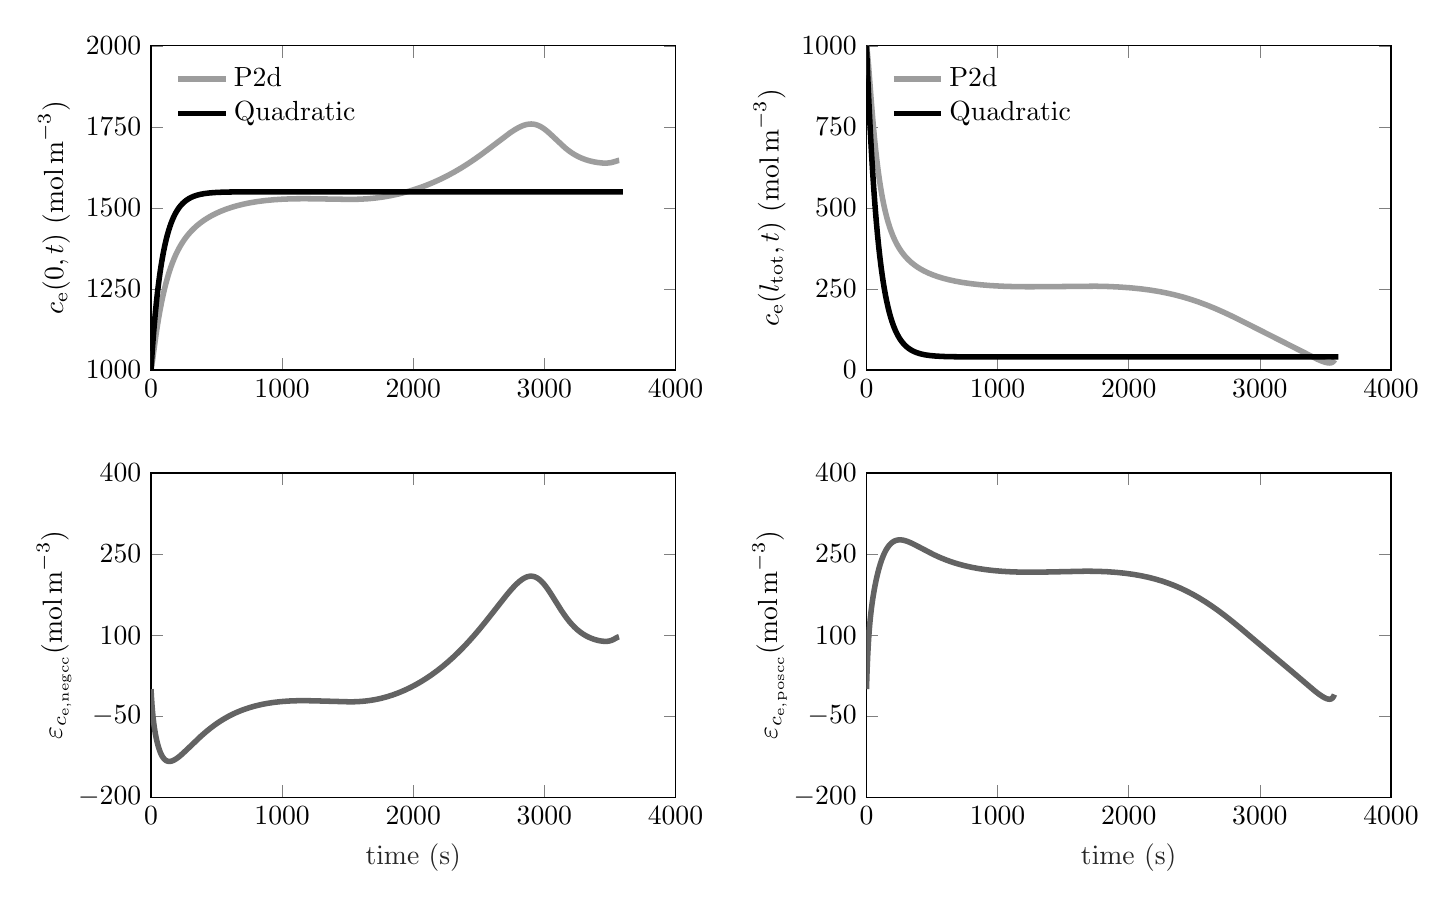
\begin{tikzpicture}

\begin{axis}[%
width=66.611mm,
height=41.169mm,
at={(0mm,54.255mm)},
scale only axis,
xmin=0,
xmax=4000,
xtick={0,1000,2000,3000,4000},
ymin=1000,
ymax=2000,
ytick={1000, 1250, 1500, 1750, 2000},
ylabel style={font=\color{white!15!black}},
ylabel={$c_{\mathrm{e}}(0,t)\  (\mathrm{mol\, m}^{-3})$},
axis background/.style={fill=white},
legend style={at={(0.03,0.97)}, anchor=north west, legend cell align=left, align=left, fill=none, draw=none},
scaled ticks=false,,
xticklabel style={/pgf/number format/1000 sep=, /pgf/number format/precision=0,/pgf/number format/fixed,/pgf/number format/fixed zerofill,},yticklabel style={/pgf/number format/1000 sep=, /pgf/number format/precision=2, /pgf/number format/fixed, }, ylabel absolute,
]
\addplot [color=mycolor1, line width=2.0pt]
  table[row sep=crcr]{%
0	1000\\
5	1011.48\\
11	1027.59\\
21	1057.49\\
37	1104.91\\
48	1134.7\\
59	1161.96\\
70	1186.88\\
81	1209.68\\
92	1230.58\\
103	1249.75\\
115	1268.89\\
127	1286.35\\
139	1302.29\\
151	1316.85\\
164	1331.24\\
177	1344.33\\
191	1357.13\\
205	1368.74\\
220	1380.03\\
235	1390.26\\
251	1400.15\\
268	1409.67\\
286	1418.78\\
306	1427.9\\
327	1436.51\\
350	1444.98\\
375	1453.22\\
402	1461.17\\
431	1468.78\\
462	1476.02\\
496	1483.04\\
532	1489.59\\
571	1495.79\\
613	1501.57\\
658	1506.88\\
706	1511.66\\
758	1515.95\\
814	1519.67\\
874	1522.77\\
939	1525.24\\
1009	1527.01\\
1086	1528.08\\
1173	1528.39\\
1278	1527.85\\
1528	1526.17\\
1597	1526.87\\
1658	1528.35\\
1715	1530.6\\
1771	1533.68\\
1827	1537.64\\
1883	1542.48\\
1939	1548.2\\
1994	1554.7\\
2049	1562.08\\
2103	1570.21\\
2156	1579.06\\
2208	1588.63\\
2260	1599.08\\
2311	1610.22\\
2362	1622.26\\
2413	1635.18\\
2465	1649.26\\
2520	1665.05\\
2583	1684.08\\
2737	1731.1\\
2771	1740.21\\
2799	1746.81\\
2823	1751.59\\
2844	1754.92\\
2864	1757.23\\
2883	1758.51\\
2901	1758.83\\
2918	1758.25\\
2935	1756.8\\
2952	1754.45\\
2969	1751.22\\
2987	1746.9\\
3006	1741.44\\
3028	1734.15\\
3055	1724.21\\
3157	1685.62\\
3184	1676.93\\
3209	1669.78\\
3234	1663.51\\
3260	1657.9\\
3287	1652.99\\
3315	1648.78\\
3345	1645.13\\
3377	1642.1\\
3411	1639.77\\
3443	1638.44\\
3470	1638.13\\
3493	1638.72\\
3513	1640.11\\
3533	1642.39\\
3567	1646.55\\
3570.66	1646.75\\
};
\addlegendentry{P2d}

\addplot [color=black, line width=2.0pt]
  table[row sep=crcr]{%
0	1000\\
8	1050.12\\
16	1094.78\\
24	1134.89\\
33	1175.42\\
42	1211.76\\
51	1244.43\\
60	1273.87\\
69	1300.43\\
78	1324.41\\
87	1346.06\\
96	1365.63\\
105	1383.31\\
115	1400.97\\
125	1416.76\\
135	1430.87\\
145	1443.48\\
155	1454.75\\
166	1465.77\\
177	1475.52\\
188	1484.13\\
200	1492.39\\
212	1499.61\\
225	1506.41\\
239	1512.7\\
254	1518.44\\
270	1523.58\\
287	1528.12\\
306	1532.26\\
327	1535.93\\
351	1539.19\\
378	1541.94\\
410	1544.29\\
448	1546.18\\
496	1547.65\\
561	1548.73\\
660	1549.4\\
858	1549.69\\
2037	1549.73\\
3599	1549.73\\
};
\addlegendentry{Quadratic}

\end{axis}

\begin{axis}[%
width=66.611mm,
height=41.169mm,
at={(90.867mm,54.255mm)},
scale only axis,
xmin=0,
xmax=4000,
xtick={0,1000,2000,3000,4000},
ymin=0,
ymax=1000,
ytick={   0,  250,  500,  750, 1000},
ylabel style={font=\color{white!15!black}},
ylabel={$c_\mathrm{e}(l_\mathrm{tot},t)\ (\mathrm{mol\, m}^{-3})$},
axis background/.style={fill=white},
legend style={at={(0.03,0.97)}, anchor=north west, legend cell align=left, align=left, fill=none, draw=none},
scaled ticks=false,,
xticklabel style={/pgf/number format/1000 sep=, /pgf/number format/precision=0,/pgf/number format/fixed,/pgf/number format/fixed zerofill,},yticklabel style={/pgf/number format/1000 sep=, /pgf/number format/precision=2, /pgf/number format/fixed, }, ylabel absolute,
]
\addplot [color=mycolor1, line width=2.0pt]
  table[row sep=crcr]{%
0	1000\\
2	995.472\\
5	986.098\\
9	970.517\\
15	942.691\\
24	895.759\\
42	801.533\\
52	754.003\\
62	710.838\\
71	675.655\\
80	643.719\\
89	614.777\\
98	588.56\\
107	564.806\\
116	543.269\\
126	521.666\\
136	502.245\\
146	484.76\\
156	468.98\\
166	454.708\\
177	440.546\\
188	427.799\\
200	415.302\\
212	404.087\\
225	393.188\\
238	383.416\\
252	373.978\\
267	364.938\\
283	356.338\\
300	348.202\\
318	340.538\\
338	332.987\\
360	325.659\\
384	318.634\\
410	311.966\\
438	305.685\\
469	299.626\\
503	293.866\\
541	288.326\\
583	283.103\\
629	278.266\\
680	273.786\\
737	269.678\\
800	266.04\\
869	262.944\\
945	260.415\\
1029	258.496\\
1123	257.235\\
1230	256.696\\
1358	256.96\\
1748	258.426\\
1846	257.471\\
1936	255.733\\
2018	253.297\\
2094	250.18\\
2165	246.404\\
2232	241.972\\
2296	236.868\\
2358	231.046\\
2418	224.549\\
2478	217.179\\
2538	208.933\\
2599	199.67\\
2662	189.218\\
2729	177.204\\
2803	163.021\\
2895	144.446\\
3439	33.1178\\
3474	27.1456\\
3499	23.7305\\
3517	22.0726\\
3531	21.5969\\
3542	22.0758\\
3551	23.3788\\
3558	25.2394\\
3564	27.6247\\
3570	30.8903\\
3570.66	31.3092\\
};
\addlegendentry{P2d}

\addplot [color=black, line width=2.0pt]
  table[row sep=crcr]{%
0	1000\\
10	901.29\\
20	811.598\\
29	738.364\\
38	671.807\\
47	611.438\\
56	556.752\\
65	507.251\\
74	462.467\\
83	421.961\\
92	385.333\\
101	352.215\\
110	322.272\\
119	295.203\\
128	270.731\\
137	248.608\\
146	228.608\\
155	210.529\\
165	192.469\\
175	176.325\\
185	161.893\\
195	148.993\\
205	137.461\\
215	127.153\\
226	117.072\\
237	108.162\\
249	99.616\\
261	92.1466\\
274	85.1122\\
288	78.6002\\
302	73.0345\\
317	67.9654\\
334	63.1625\\
352	58.9826\\
372	55.2281\\
395	51.8332\\
421	48.9153\\
451	46.453\\
487	44.408\\
532	42.7787\\
591	41.5774\\
676	40.7904\\
828	40.3865\\
1351	40.297\\
3599	40.2968\\
};
\addlegendentry{Quadratic}

\end{axis}

\begin{axis}[%
width=66.611mm,
height=41.169mm,
at={(0mm,0mm)},
scale only axis,
xmin=0,
xmax=4000,
xtick={0,1000,2000,3000,4000},
xlabel style={font=\color{white!15!black}},
xlabel={time (s)},
ymin=-200,
ymax=400,
ytick={-200,  -50,  100,  250,  400},
ylabel style={font=\color{white!15!black}},
ylabel={$\varepsilon_{c_{\mathrm{e,negcc}}} (\mathrm{mol\, m}^{-3})$},
axis background/.style={fill=white},
scaled ticks=false,,
xticklabel style={/pgf/number format/1000 sep=, /pgf/number format/precision=0,/pgf/number format/fixed,/pgf/number format/fixed zerofill,},yticklabel style={/pgf/number format/1000 sep=, /pgf/number format/precision=2, /pgf/number format/fixed, }, ylabel absolute,
]
\addplot [color=mycolor2, line width=2.0pt, forget plot]
  table[row sep=crcr]{%
0	0\\
4	-16.7879\\
8	-30.8604\\
12	-42.6054\\
16	-52.4801\\
20	-60.9172\\
24	-68.2618\\
29	-76.2826\\
34	-83.3141\\
40	-90.7277\\
46	-97.2286\\
52	-102.956\\
58	-108.006\\
64	-112.447\\
71	-116.935\\
78	-120.745\\
85	-123.946\\
92	-126.598\\
100	-129.025\\
108	-130.879\\
116	-132.226\\
125	-133.21\\
135	-133.732\\
145	-133.747\\
156	-133.263\\
169	-132.134\\
183	-130.379\\
199	-127.841\\
218	-124.285\\
242	-119.223\\
275	-111.684\\
380	-87.3521\\
418	-79.2768\\
453	-72.3659\\
488	-65.9941\\
523	-60.1682\\
558	-54.8783\\
594	-49.9747\\
631	-45.4724\\
669	-41.3785\\
709	-37.6062\\
750	-34.264\\
793	-31.2786\\
839	-28.6178\\
887	-26.3693\\
938	-24.5079\\
992	-23.062\\
1050	-22.0367\\
1113	-21.456\\
1183	-21.3506\\
1265	-21.7717\\
1526	-23.5612\\
1580	-23.1206\\
1628	-22.2229\\
1673	-20.8735\\
1717	-19.0355\\
1760	-16.7229\\
1803	-13.8929\\
1846	-10.5446\\
1889	-6.67745\\
1932	-2.28814\\
1975	2.62922\\
2017	7.94948\\
2059	13.7901\\
2101	20.1626\\
2142	26.9094\\
2183	34.1897\\
2223	41.8196\\
2263	49.9816\\
2303	58.6858\\
2342	67.7008\\
2381	77.2393\\
2421	87.5613\\
2462	98.6915\\
2504	110.636\\
2550	124.277\\
2605	141.163\\
2710	173.545\\
2742	182.767\\
2768	189.72\\
2790	195.071\\
2810	199.389\\
2828	202.732\\
2844	205.196\\
2859	207.011\\
2874	208.292\\
2888	208.962\\
2902	209.087\\
2915	208.689\\
2928	207.777\\
2941	206.342\\
2954	204.385\\
2967	201.916\\
2981	198.711\\
2995	194.978\\
3010	190.455\\
3027	184.775\\
3047	177.514\\
3075	166.721\\
3127	146.598\\
3151	137.956\\
3172	130.946\\
3192	124.817\\
3212	119.25\\
3231	114.489\\
3251	110.016\\
3271	106.068\\
3292	102.448\\
3314	99.1837\\
3337	96.2918\\
3362	93.6889\\
3388	91.5225\\
3414	89.8807\\
3439	88.8248\\
3461	88.4053\\
3480	88.5476\\
3497	89.1998\\
3512	90.286\\
3527	91.8914\\
3549	94.8767\\
3563	96.5169\\
3569	96.9425\\
};
\end{axis}

\begin{axis}[%
width=66.611mm,
height=41.169mm,
at={(90.867mm,0mm)},
scale only axis,
xmin=0,
xmax=4000,
xtick={0,1000,2000,3000,4000},
xlabel style={font=\color{white!15!black}},
xlabel={time (s)},
ymin=-200,
ymax=400,
ytick={-200,  -50,  100,  250,  400},
ylabel style={font=\color{white!15!black}},
ylabel={$\varepsilon_{c_{\mathrm{e,poscc}}} (\mathrm{mol\, m}^{-3})$},
axis background/.style={fill=white},
scaled ticks=false,,
xticklabel style={/pgf/number format/1000 sep=, /pgf/number format/precision=0,/pgf/number format/fixed,/pgf/number format/fixed zerofill,},yticklabel style={/pgf/number format/1000 sep=, /pgf/number format/precision=2, /pgf/number format/fixed, }, ylabel absolute,
]
\addplot [color=mycolor2, line width=2.0pt, forget plot]
  table[row sep=crcr]{%
0	0\\
3	23.1751\\
6	42.7981\\
9	59.7628\\
13	78.9848\\
17	95.0498\\
21	108.643\\
25	120.333\\
29	130.57\\
34	141.828\\
39	151.796\\
45	162.483\\
51	172.1\\
58	182.258\\
65	191.483\\
72	199.917\\
80	208.706\\
88	216.696\\
96	223.963\\
104	230.569\\
112	236.563\\
121	242.629\\
130	248.03\\
139	252.82\\
148	257.043\\
157	260.735\\
167	264.263\\
177	267.239\\
188	269.929\\
199	272.068\\
211	273.839\\
223	275.088\\
236	275.926\\
250	276.309\\
265	276.213\\
282	275.581\\
301	274.348\\
323	272.397\\
350	269.468\\
388	264.774\\
513	248.956\\
559	243.852\\
604	239.387\\
649	235.443\\
696	231.854\\
745	228.643\\
797	225.77\\
852	223.265\\
911	221.111\\
974	219.343\\
1042	217.966\\
1116	217.001\\
1197	216.477\\
1289	216.421\\
1402	216.905\\
1676	218.312\\
1760	218.059\\
1836	217.313\\
1907	216.096\\
1973	214.447\\
2035	212.379\\
2093	209.93\\
2148	207.094\\
2201	203.837\\
2252	200.175\\
2301	196.134\\
2349	191.65\\
2396	186.735\\
2443	181.288\\
2489	175.436\\
2536	168.925\\
2583	161.886\\
2631	154.172\\
2681	145.604\\
2734	135.977\\
2791	125.08\\
2857	111.913\\
2959	90.9456\\
3093	63.5293\\
3248	31.8709\\
3419	-3.40536\\
3452	-9.51159\\
3476	-13.4575\\
3495	-16.0901\\
3510	-17.6881\\
3522	-18.4989\\
3532	-18.6943\\
3540	-18.3842\\
3547	-17.6248\\
3553	-16.4744\\
3558	-15.0573\\
3563	-13.1274\\
3568	-10.5996\\
3569	-10.0164\\
};
\end{axis}
\end{tikzpicture}%






